\begin{frame}{6面体要素が切れる形状の条件}
  \begin{table}[hbtp]
      \caption{3次元構造解析で使われる主なメッシュ要素(一部)<参考文献\cite{handbook}>}
      \vspace{-5mm}
      \begin{tabular}{|r|c|c|c|} % 表は項目名を右寄せ、データを中寄せ
          \hline
          名称       & 4面体2次要素 & 6面体1次要素 & 4面体1次要素 \\
          \hline
          接点配置   & 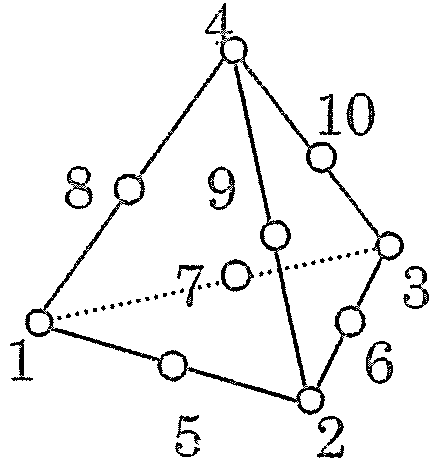
\includegraphics[keepaspectratio]{work/images/tet10.png}
                     & 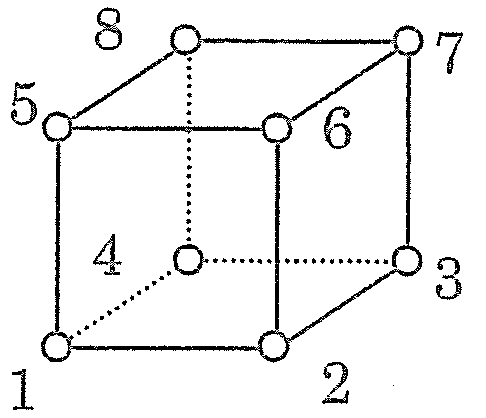
\includegraphics[keepaspectratio]{work/images/hex8.png} 
                     & 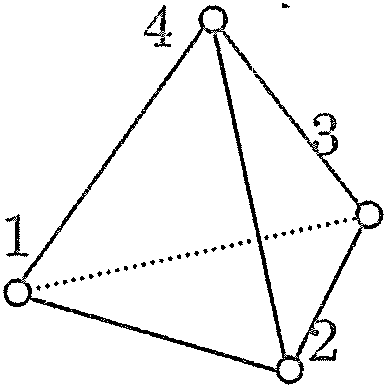
\includegraphics[keepaspectratio]{work/images/tet4.png}  \\
          \hline
          メリット   & 任意の形状で切れる & 見た目が美しい & 無 \\
          \hline
          デメリット & 多少見た目が悪い   & 形状に人間の介入が必要 & 硬い \\
          \hline
          評価       &   〇               & ◎              & × \\
          \hline
    \end{tabular}
  \end{table}
  %
\end{frame}
